\documentclass[a4paper,12pt]{report}
\usepackage[utf8]{inputenc}
\usepackage{amsmath}
\usepackage{graphicx}
\usepackage{listings}
\usepackage{tikz}
\usepackage[T1]{fontenc}
\usepackage{color}
\usetikzlibrary{arrows,automata}
\definecolor{pythonred}{rgb}{0.6,0,0} % for strings
\definecolor{pythongreen}{rgb}{0.25,0.5,0.35} % comments
\definecolor{pythonpurple}{rgb}{0.5,0,0.35} % keywords
	\definecolor{pythondocblue}{rgb}{0.25,0.35,0.75} % javadoc
	 
	\lstset{language=python,
	basicstyle=\ttfamily,
	keywordstyle=\color{pythonpurple}\bfseries,
	stringstyle=\color{pythonred},
	commentstyle=\color{pythongreen},
	morecomment=[s][\color{pythondocblue}]{/**}{*/},
	numbers=left,
	numberstyle=\tiny\color{black},
        stepnumber=2,
	numbersep=10pt,
	tabsize=4,
	showspaces=false,
	showstringspaces=false}

% Title Page

 \title{\bfseries\huge \textcolor{purple}{\underline {EEP702-Software Lab}} \\{\textcolor{blue}{Assignment 2 : String Occurrence Count  Using Shell Script and C++ program  }}}
\author{\bfseries\large\textcolor{black}  {Harshit Kumar Gupta}\\ {\textcolor{black} {2013EET2369}}\\

\includegraphics[width=3cm,height=3.4cm]{./iit.png}\\\noindent Computer Technology\\
\noindent Department Of Electrical Engineering\\IIT DELHI}
% iit.png: 282x282 pixel, 72dpi, 9.95x9.95 cm, bb=0 0 282 282
\begin{document}
\maketitle
\tableofcontents


\chapter{\textcolor{blue}{\underline {PROBLEM STATEMENT}}}
\noindent String manipulation using shell scripts - writing a program (called NumOfOccurrences) to find how many 
times a substring s2 occurs in a bigger string s1\\\\
Using csh, sed and awk (either separately or together - see pipes and |tee connectors to send the output of one program into another)\\\\
1. Part (a)\\Find the total number of occurrences of a substring s2 to be entered by the user. Logically divide the string s1 into 'm' number of even partitions and parallely search to count the total number of 
occurrences of s2 parallely using threads, where 'm' is the number of threads to be entered by the user.\\\\
2. Part (b)\\
Let the length of string s1 [denoted as len(s1) ] be n1 and number of threads be m, then the length of each partition would be (n1/m) and n2 = len(s2) ( < (n1/m)) During runtime, print using an external subroutine StringPrint(*char s) the 'id' of thread in which the substring s2 is found. Each thread will find the occurrence in its local string partition. IPC and message 
queues can be used for communication among threads, and finally print the total number of occurrences of s2 in s1.\\\\
3. Part (c)\\
Repeat the above using any one of the languages C / C++ / Java
\begin{center}
\chapter{\textcolor{blue}{\underline {ABSTRACT}}}
\end{center}
\noindent This report includes description on two codes designed for above two problems. The first code deals with string manipulation in bash scripts
 and the second program which is in C++, deals with string manipulation using the concept of threading. Threading gives us an
 upper edge while processing concurrently the string matching algorithm to provide us the output in a very efficient and fast manner.
 The string s1 contains the text and string s2 contains the search texts, the string s1 is divided into many parts as per the no of threads is provided
 and concurrently starting the process of matching the desired string s2 in s1.

\begin{center}
\chapter{\textcolor{blue}{\underline {INTRODUCTION}}}
\end{center}
\noindent \textbf The first program which is a bash script computes the search and prints no. of occurrence of string s2 in s1.\\

    Bash is a Unix shell written by Brian Fox for the GNU Project as a free software replacement for the Bourne shell (sh). Released in 1989,it has been 
distributed widely as the shell for the GNU operating system and as a default shell on Linux and Mac OS X.Bash is a command processor, typically run in a text window, allowing the user to type commands which cause actions. Bash can also read commands from a file, called a script. Like all Unix shells, it supports filename wildcarding, 
piping, here documents, command substitution, variables and control structures for condition-testing and iteration.\\\\
    
      The second program is the same as the first but the only difference is that the second program is in C++ code and concepts of threads are used in it to execute the search in a very efficient time.
    Multi-threading is a widespread programming and execution model that allows multiple threads to exist within the context of a single process. These threads share the process' resources, but are able to execute independently. 
    The threaded programming model provides developers with a useful abstraction of concurrent execution. Multi-threading can also be applied to a single process to enable parallel execution on a multiprocessing system.
  This advantage of a multithreaded program allows it to operate faster on computer systems that have multiple CPUs, CPUs with multiple cores, or across a cluster of machines, because the threads of the program naturally lend themselves to truly concurrent execution.
\begin{center}
\chapter{\textcolor{blue}{\underline {SPECIFICATIONS AND ASSUMPTIONS}}}
\end{center}
\section*{Specifications}

\begin{enumerate}
 \item A substring s2 is input by the user in either of the following ways (a) either the user types s2 on the terminal or (b) from the shell prompt in two ways (again!)
\begin{enumerate}
 \item INVOCATION 1 :  NumOfOccurrences s2 (only one string is given and it is understood as s2,s1 is hardcoded in the program)
  \item INVOCATION 2 :  NumOfOccurrences s1 s2 (both strings are specified on the command line and the sequence determines which s s1 and which is s2)
\end{enumerate}
\item The output of StringPrint(.) looks moreover like this:
<current UTC time> <id of thread where s2 is found> [n times]\\
Total embeddings of s2 in s1 = no of occurrences.


\end{enumerate}


 
\section*{Assumptions}

\begin{enumerate}
 \item  The first string can be a text file containing string s1 of alphanumeric characters.
\item The second string s2 can be given as argument or can be taken as input from the user.
\item The last line of output only the words s2 and s1 are bold (emphasized) when the sentence is printed on the terminal.

\end{enumerate}
 
\begin{center}
\chapter{\textcolor{blue}{\underline {LOGIC USED/METHODOLOGY}}}
\end{center}
The methodology that is used for developing the program is defined below:

\begin{enumerate}
\item First the string s1 and s2 is fed as input to the program as command line argumants.
\item we check if size of substring is grater than bigger string tehn we exit.
\item We start from first character of main string and match with first character of substring .if match then increment postion by 1 in both string
\item if no mismatch is found and substring is completed then we increment no of occurrences.
\item if mismatch is found then starting postion for matching in main string is incremented by one.
\item We repeat the above procedure till we reach at end of first string.
\\
\item To achieve parallism in matching procedure we can use threading in c++ using pthread library.
\item To achieve parallism in bash program we can run matching procedure as backgroud process .OS schedules background process in paralllel. 
\end{enumerate}




\begin{center}
\chapter{\textcolor{blue}{\underline {EXECUTION INSTRUCTIONS}}}

\begin{enumerate}
 \item For first program in bash following instructions are used.
 \begin{enumerate}
  \item chmod 777 parallel-count.sh
  \item parallel-count.sh <s1> <s2> 
 \end{enumerate}
\item For second program in C++ following instructions are used.
\begin{enumerate}
 \item g++ -Wall  NoOfOccurrences.cpp -lpthread
\item We can also use makefile by --- make -f Makefile1
\item to excute the program use--
\\NoOfOccurrences <s1> <s2> 
\end{enumerate}

\end{enumerate}
Repeat the above instructions for different input strings of s1 and s2.
\end{center}

\begin{center}
\chapter{\textcolor{blue}{\underline {FLOWCHART}}}


 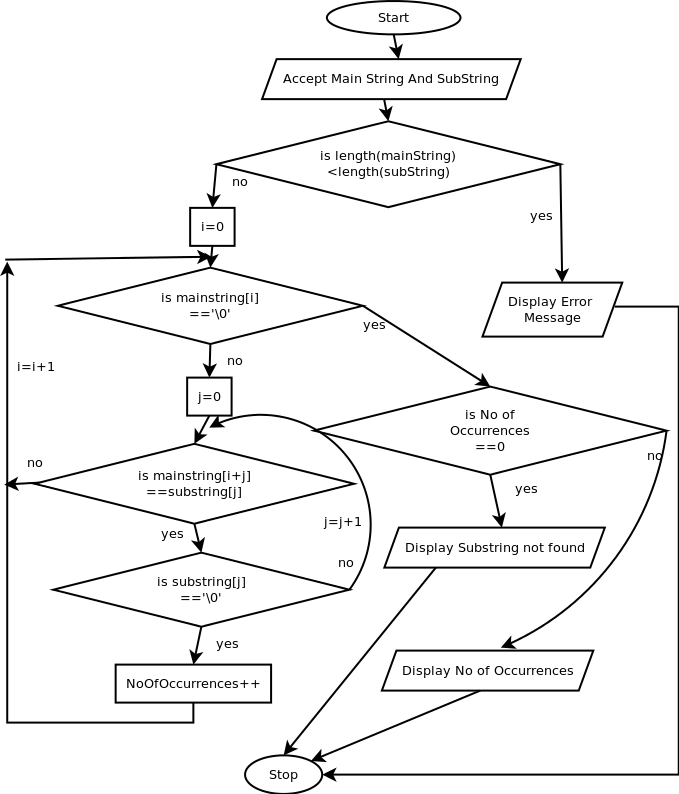
\includegraphics[width=15 cm,height=13 cm]{./Diagram1.png}
 % flowchart.png: 668x744 pixel, 72dpi, 23.57x26.25 cm, bb=0 0 668 744
\end{center}


\begin{center}
\chapter{\textcolor{blue}{\underline {OUTPUT}}}

 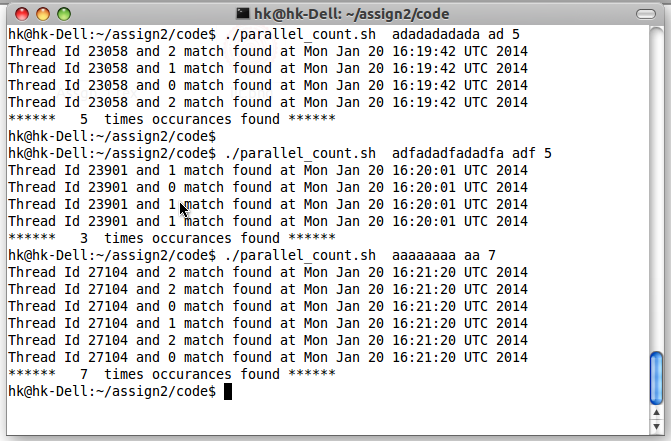
\includegraphics[width=13 cm,height=13 cm]{./Screenshot1.png}
 % flowchart.png: 668x744 pixel, 72dpi, 23.57x26.25 cm, bb=0 0 668 744

Output of Bash Script
\end{center}
\begin{center}
 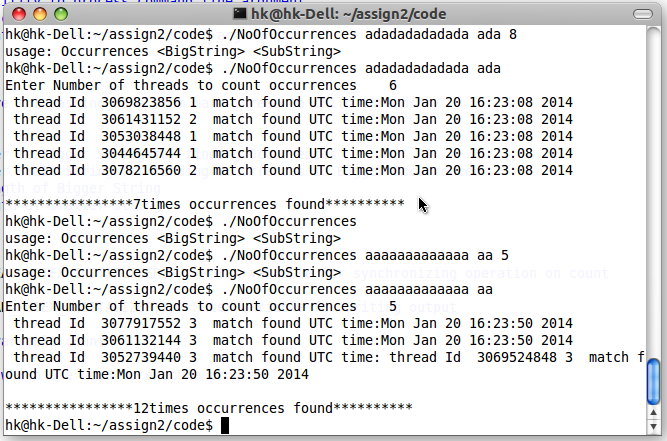
\includegraphics[width=13 cm,height=13 cm]{./Screenshot2.png}
 % flowchart.png: 668x744 pixel, 72dpi, 23.57x26.25 cm, bb=0 0 668 744

Output of C++ program
\end{center}



\begin{center}
\chapter{\textcolor{blue}{\underline {RESULTS AND CONCLUSIONS}}}\end{center}

\noindent In both the cases the value output of the Bash Script  and c++code is displayed on the user screen using the echo or cout command for the strings. 
\noindent In both the cases the output comes out to  be as expected and is verified for all the conditions.



\end{document}    